%_________________________________________Heading_______________________________________________%

\documentclass[11pt]{article}
% #1-Asignatura
% #2-Curso
% #3-Nombre
% #4-Link
% #5-Foto

\newcommand{\portada}[5]{
    \begin{titlepage}
        \begin{center}
            \vspace*{0.5cm}
            
            % Titulo con #1 lo mas grande posible
            {\Huge \textbf{#1}}

            
            \vspace{0.5cm}
            \LARGE
            Curso #2 
            
            \vspace{1cm}
            
            \Huge{\textbf{Grupo Viterbi}}

            \vspace{1cm}
            
\includegraphics[width=0.6\textwidth]{assets/Img/UGR-Logo.png}
            
            \vspace{0.5cm}

            \huge
            PRÁCTICA 5- PROGRAMACIÓN DINÁMICA
            
            \Large
            \vspace{1cm}
            \textbf{Integrantes:}  \\ 
             % Array con los nombres de los integrantes y el correo
             \begin{center}
                \begin{tabular}{c c }
                    \textbf{Miguel Ángel De la Vega Rodríguez} & miguevrod@correo.ugr.es \\
                    \textbf{Alberto De la Vera Sánchez} & joaquinrojo724@correo.ugr.es \\
                    \textbf{Joaquín Avilés De la Fuente} & adelaveras01@correo.ugr.es \\
                    \textbf{Manuel Gomez Rubio} & e.manuelgmez@go.ugr.es \\
                    \textbf{Pablo Linari Perez} & e.pablolinari@go.ugr.es
                \end{tabular}
             \end{center}
            \vspace{0.8cm}
            
            
            \large
             \vspace{1cm}
            Facultad de Ciencias UGR\\
            Escuela Técnica Ingeniería Informática UGR\\
            Granada\\
            #2 
            
        \end{center}
    \end{titlepage}
}



\usepackage{assets/formulas}
\usepackage{float}
\hbadness=10000 % Suppress Underfull \hbox warnings

%_________________________________________Indice:_______________________________________________%
\begin{document}                                                
\portada{Algorítmica}{2023-2024}{Miguel Ángel De la Vega Rodríguez}{https://github.com/Miguevrgo/}{github.png}

\tableofcontents % Índice

\newpage %Salto de pagina tras el Indice

%________________________________________Documento:_____________________________________________%
\section{Participación}
\begin{itemize}
    \item \textbf{Miguel Ángel De la Vega Rodríguez:} 20\%
    \begin{itemize}
        \item Plantilla y estructura del documento \LaTeX
        \item Cómputo de la eficiencia de los algoritmos (Resultados y Ajuste)
    \end{itemize}
    \item \textbf{Joaquín Avilés De la Fuente:} 20\%
    \begin{itemize}
        \item Descripción del Objetivo de la pŕactica
        \item Diseño del estudio
    \end{itemize}
    \item \textbf{Alberto De la Vera Sánchez: } 20\%
    \item \textbf{Manuel Gomez Rubio} 20\%
    \item \textbf{Pablo Linari Pérez:} 20\%
    \begin{itemize}
        \item Estudio y comparación de las gráficas
        \item Diseño del estudio
    \end{itemize}
\end{itemize}

\section{Equipo de trabajo}

\begin{itemize}
    \item \textbf{Miguel Ángel De la Vega Rodríguez:} (Ordenador donde se ha realizado el computo)
        \begin{itemize}
            \item AMD Ryzen 7 2700X 8-Core
            \item 16 GB RAM DDR4 3200 MHz
            \item NVIDIA GeForce GTX 1660 Ti 
            \item 1 TB SSD NvMe 
        \end{itemize}
\end{itemize}

\section{Objetivos}
    En esta práctica, se han implementado los siguientes algoritmos de ordenación: \textbf{quicksort, mergesort, inserción, burbuja,}
    y \textbf{selección}. Además, se han implementado los algoritmos de \textbf{Floyd}, que calcula el costo del camino mínimo entre cada par de nodos 
    de un grafo dirigido, de \textbf{Fibonacci}, que calcula los números de la sucesión de Fibonacci , y de \textbf{Hanoi}, que resuelve el famoso 
    problema de las torres de Hanoi. Se ha aplicado la siguiente metodología:
    \begin{itemize}
        \item En primer lugar, aunque tenemos la eficiencia teórica de estos algoritmos, se realizarán los calculos necesarios para demostrar
        como se obtiene dicha eficiencia utilizando los distintos métodos estudiados en teoría. \\
        
        \item En segundo lugar, se pasará al estudio empírico de los algoritmos de ordenación de vectores para distintos tipos de datos, es decir, 
        para datos tipo \textbf{int}, \textbf{float}, \textbf{double} y \textbf{string}. Posteriormente, se creará las gráficas para
        cada algoritmo en las que visualizaremos el tiempo de ejecución en función del tamaño del vector y del tipo de dato. Finalmente 
        para esta parte, se hara un calculo de \textbf{eficiencia híbrida} que se basa en ajustar la gráfica obtenida a la función de su eficiencia
        teórica por mínimos cuadrados, obteniendo por tanto los literales de dicha función que ajustan la gráfica.\\
        
        \item En tercer lugar, se hará el estudio de los otros tres algoritmos de forma similar, es decir, se estudiará la eficiencia
        de estos de modo empírica, cuyo estudio se mostrará en las gráficas, y se calculará la eficiencia híbrida de estos, a partir
        de la eficiencia teórica.\\     
    \end{itemize}
\section{Diseño del estudio}

    Los estudios empíricos han sido realizados en el ordenador con las características mencionadas anteriormente.
    Además, hemos realizado el estudio empírico de forma aislada para el algoritmo de ordenación de vectores
    quicksort en los distintos ordenadores de los participantes del grupo para ver como afectan las características
    hardware de cada ordenador en el tiempo de ejecución, cuyas gráficas se mostrarán en la sección de Algoritmos. \\
    En ambos casos se ha hecho uso del sistema operativo Linux, concretamente de Debian, y se ha utilizado el
    compilador gcc para la compilación de los programas  con el flag -Og para la optimización.
    \subsection{Algoritmos de ordenación de vectores}
    Para los algoritmos de ordenación se han usado entradas de datos de tipo int, float, double y string mientras que para los algoritmos de Hanoi, Floyd  y Fibonnaci solo se han usado entradas de tipo int 
    ya que no tendría sentido usar entradas de otro tipo. 
    \begin{itemize}
        \item En los algoritmos con eficiencia  \(O(n^2)\) como los de Burbuja, Selección e Inserción los saltos usados entre los tipos de datos int, float y double generados aleatoriamente son de 5000 en 5000 empezando con una muestra de 5000 datos y llegando a
        un máximo de 125000 datos.
        \item En los lagoritmos con eficiencia \(O (n\log(n))\) como el mergesort o el quicksort los saltos usados entre los tipos de datos int, float y double generados aleatoriamente son de 50000 en 50000 empezando con una muestra de 50000 datos y llegando a
        un máximo de 1250000 datos.
    \end{itemize}

    \subsection{Otros algoritmos}
    En los algoritmos restantes se han usado datos de tipo int generados aleatoriamente y proporcionados en la siguiente medida:
    \begin{itemize}
        \item Para el algoritmo de Floyd  que es de orden \(O(n^3)\) se han usado enteros aleatorios desde 50 hasta 1250 con saltos de 50 en 50.
        \item Para el algoritmo de Fibonnaci  que es de orden \(O((\frac{1+\sqrt{5}}{2})^n\)) se han usado enteros aleatorios desde 50 hasta 1250 con saltos de 50 en 50.
        \item Para el algoritmo de Hanoi que es de orden \(O(2^n)\) se han usado enteros aleatorios desde 3 hasta 33 con saltos de 50 en 50. 
    \end{itemize}

    Por último para el tipo de dato string se han extraido las muestras del archivo \textit{quijote.txt} para simular una generación aleatoria de palabras, 
    esta entrada de datos no ha sido totalmente aleatoria ya que al usar un lenguaje determinado para el texto, en este caso el español, se repiten con mas frecuencia algunas palabras por tanto esto se verá 
    reflejado en el comportamiento de los  algoritmos. En este caso el Quijote tiene un total de 202308 palabras por lo que se comenzará con una muestra de 12308 palabras con saltos de 
    10000 en 10000 hasta llegar a 202308 palabras.
    \subsection{Scripts usados para la ejecución}
    \begin{itemize}
        \item \textbf{[AutoCompile.sh]} Este script se encarga de compilar todos los ficheros en una misma carpeta con las mismas
        opciones de compilación, para garantizar la máxima igualdad posible entre cada algoritmo y organizar la estructura de 
        ficheros.
        \item \textbf{[AutoFinal.sh]} Este script es el encargado de ejecutar todos los algoritmos varias veces con las opciones respectivas para cada uno,
        el resultado se pasa por un programa AutoMedia.py que se encarga de realizar la media de las ejecuciones de los algoritmos,
        este resultado es guardado en una carpeta llamada Resultados de la que posteriormente el mismo script genera las graficas
        de cada algoritmo.
        \item \textbf{[AutoIndividual.sh]} Este script es como el descrito previamente pero unicamente ejecuta un script, esto ha sido útil para hacer
        pruebas sin la necesidad de esperar la gran cantidad de tiempo que requiere la ejecución de todos los algoritmos.
    \end{itemize}
    
\section{Algoritmos}
    Esta sección esta dedicada a mostrar los resultados obtenidos en el estudio de los algoritmos,
    la estructura seguida para mostrar los resultados consiste en mostrar, para cada algoritmo, los tiempos 
    de ejecución, junto con las gráficas obtenidas y los ajustes correspondientes. Previo a ello, se analizará
    en cada caso teoricamente la eficiencia prevista para cada algoritmo.

    \subsection{Estudio teórico}
        En esta sección se calculará la eficiencia teórica de cada algoritmo, es decir, la eficiencia que se espera al hacer el
        estudio empírico de cada algoritmo. Para ello, se utilizarán los métodos estudiados en teoría.
        \subsection*{Algoritmo de ordenación Burbuja}
        Utilizaremos el siguiente fragmento de código para estudiar su eficiencia, pues es el utilizado en la práctica
        \begin{lstlisting}
            void burbuja(int T[], int inicial, int final)
            {
            int i, j;
            int aux;
            for (i = inicial; i < final - 1; i++)
                for (j = final - 1; j > i; j--)
                if (T[j] < T[j - 1])
                {
                    aux = T[j];
                    T[j] = T[j - 1];
                    T[j - 1] = aux;
                }
            }
        \end{lstlisting}
        El trozo de código dentro del bucle interno, es decir, de la línea 7 a la 12 tiene eficiencia $O(1)$ y por tanto
        tiene un tiempo de ejecución constante que anotaremos como $a$. Además, este trozo de código se ejecuta
        en concreto $(final-1)-(i+1) +1$ veces, es decir, $final-i+1$ veces. Es claro que la ejecución de la línea 3 y 4 
        y las comparaciones, inicializaciones y actualizaciones de los bucles tienen eficiencia $O(1)$. Sabiendo esto y que 
        el número de veces que se ejecute el bucle interno depende del externo tenemos entonces la siguiente fórmula 
        \begin{equation*}
            \sum_{i=inicial}^{final-2} \sum_{j=i+1}^{final-1}a 
        \end{equation*}
        Tomaremos $final =  n$ e $inicial = 1$ para simplificar el cálculo y veamos que obtenemos ahora
        \begin{equation*}\begin{split}
            \sum_{i=1}^{n-2} \sum_{j=i+1}^{n-1}a= a \cdot \sum_{i=1}^{n-2} \sum_{j=1}^{n-i-1}1
            & = a \cdot \sum_{i=1}^{n-2} (n-i-1) a \cdot ( n\sum_{i=1}^{n-2} 1 - \sum_{i=1}^{n-2} i - \sum_{i=1}^{n-2} 1)= \\
            &= a \cdot ( n(n-2) - \frac{(n-2)(n-1)}{2} - (n-2))= a \cdot ( n^2-2n - \frac{n^2-3n+2}{2} - n+2)=\\
            &= a \cdot (\frac{n^2}{2}-\frac{3}{2}n+1)= \frac{n^2}{2}a-\frac{3}{2}na+a
        \end{split}\end{equation*}
        Es claro que $\frac{n^2}{2}a-\frac{3}{2}na+a \in O(n^2)$ y por tanto la eficiencia teórica del algoritmo de burbuja es $O(n^2)$.

        \subsection*{Algoritmo de ordenación Inserción}
        Utilizaremos el siguiente fragmento de código para estudiar su eficiencia, pues es el utilizado en la práctica
        \begin{lstlisting}
            void insercion(int T[], int inicial, int final)
            {
              int i, j;
              int aux;
              for (i = inicial + 1; i < final; i++) {
                j = i;
                while ((T[j] < T[j-1]) && (j > 0)) {
                  aux = T[j];
                  T[j] = T[j-1];
                  T[j-1] = aux;
                  j--;
                };
              };
            }
            
        \end{lstlisting}
        El trozo de código dentro del bucle interno, es decir, de la línea 8 a la 10 tiene eficiencia $O(1)$ y por tanto
        tiene un tiempo de ejecución constante que anotaremos como $a$. Dicho trozo de código se ejecutará en el peor de los casos
        $i-(0-1)+1=i$ veces, mientras que el bucle while se ejecutará $(final-1)-(inicial+1)+1=final-inicial-1$ veces.
        Sabiendo que la ejecución de la línea 3 y 4 y las comparaciones, inicializaciones y actualizaciones de los bucles tienen eficiencia $O(1)$, 
        tenemos la siguiente fórmula
        \begin{equation*}
            \sum_{i=inicial+1}^{final-1} \sum_{j=1}^{i}a
        \end{equation*}
        Tomaremos $final =  n$ e $inicial = 1$ para simplificar el cálculo y veamos que obtenemos ahora
        \begin{equation*}
            \sum_{i=2}^{n-1} \sum_{j=1}^{i}a= a \cdot \sum_{i=1}^{n-2} \sum_{j=1}^{i}1= a \cdot \sum_{i=1}^{n-2} i
            = a \cdot \frac{(n-2)(n-1)}{2}=\frac{n^2}{2}a-\frac{3n}{2}a+a 
        \end{equation*}
        Es claro que $\frac{n^2}{2}a-\frac{3}{2}na+a \in O(n^2)$ y por tanto la eficiencia teórica del algoritmo de inserción es $O(n^2)$.
        
        \subsection*{Algoritmo de ordenación Selección}
        Utilizaremos el siguiente fragmento de código para estudiar su eficiencia, pues es el utilizado en la práctica
        \begin{lstlisting}
            void seleccion(int T[], int inicial, int final)
            {
              int i, j, indice_menor;
              int menor, aux;
              for (i = inicial; i < final - 1; i++) {
                indice_menor = i;
                menor = T[i];
                for (j = i; j < final; j++)
                  if (T[j] < menor) {
                    indice_menor = j;
                    menor = T[j];
                  }
                aux = T[i];
                T[i] = T[indice_menor];
                T[indice_menor] = aux;
              };
            }
        \end{lstlisting}
        El trozo de código dentro del bucle interno, es decir, de la línea 9 a la 14 tiene eficiencia $O(1)$ y por tanto
        tiene un tiempo de ejecución constante que anotaremos como $a$. Este trozo de código se ejecutará en el peor de los casos
        $(final-1)-i+1=final-i$ veces, mientras que el bucle for interno se ejecutará $(final-1-1)-inicial+1=final -inicial-1$ veces.
        Sabiendo que la ejecución de las líneas 3, 4, 6, 7 y las comparaciones, inicializaciones y actualizaciones de los 
        bucles tienen eficiencia $O(1)$, tenemos la siguien fórmula
        \begin{equation*}
            \sum_{i=inicial}^{final-2} \sum_{j=i}^{final-1}a 
        \end{equation*}
        Tomaremos $final =  n$ e $inicial = 1$ para simplificar el cálculo y veamos que obtenemos ahora
        \begin{equation*}\begin{split}
            \sum_{i=1}^{n-2} \sum_{j=i}^{n-1}a= a \cdot \sum_{i=1}^{n-2} \sum_{j=1}^{n-1-(i-1)}1
            & = a \cdot \sum_{i=1}^{n-2} \sum_{j=1}^{n-i}1=a \cdot \sum_{i=1}^{n-2} n-i= a \cdot (n\sum_{i=1}^{n-2}1 - \sum_{i=1}^{n-2}i) \\
            & = a \cdot(n(n-2)-\frac{(n-2)(n-1)}{2})= a \cdot (n^2-2n-\frac{n^2-3n+2}{2})= a \cdot (\frac{n^2}{2}-\frac{n}{2}+1) \\
            & = \frac{n^2}{2}a-\frac{n}{2}a+a
        \end{split}\end{equation*}
        Es claro que $\frac{n^2}{2}a-\frac{n}{2}a+a \in O(n^2)$ y por tanto la eficiencia teórica del algoritmo de inserción es $O(n^2)$.

        \subsection*{Algoritmo de ordenación Mergesort}
        Utilizaremos el siguiente fragmento de código para estudiar su eficiencia, pues es el utilizado en la práctica
        \begin{lstlisting}
  
        static void fusion(int T[], int inicial, int final, int U[], int V[])
        {
            int j = 0;
            int k = 0;
            for (int i = inicial; i < final; i++){
                if (U[j] < V[k]) {
                    T[i] = U[j];
                    j++;
                } else{
                    T[i] = V[k];
                    k++;
                };
            };
        }

        void mergesort(int T[], int inicial, int final)
        {
            if (final - inicial < UMBRAL_MS){
                insercion(T, inicial, final);
            } else {
                int k = (final - inicial)/2;

                int * U = new int [k - inicial + 1];
                assert(U);
                int l, l2;
                for (l = 0, l2 = inicial; l < k - inicial; l++, l2++)
                    U[l] = T[l2];
                U[l] = INT_MAX;

                P * V = new P [final - k + 1];
                assert(V);
                for (l = 0, l2 = k; l < final - k; l++, l2++)
                    V[l] = T[l2];
                V[l] = INT_MAX;

                mergesort_lims(U, 0, k - inicial);
                mergesort_lims(V, 0, final - k);
                fusion(T, inicial, final, U, V);
                delete [] U;
                delete [] V;
            };
        }
            
        \end{lstlisting}
        Destacar que tomaremos $final=n$ e $inicial=0$. Es claro que en el caso de $n=final-incial<\nobreak UMBRAL\_MS$ 
        la eficiencia del algoritmo en el peor caso es $O(UMBRAL\_MS^2)$, es decir, constante, por tanto, nos centraremos en el caso en el que $n\geq UMBRAL\_MS$.
        En este caso, el algoritmo se divide en dos partes, la primera parte es la creación de los vectores $U$ y $V$ y la segunda parte es la
        llamada recursiva a la función mergesort y el resto de código. \\
        La primera parte la podemos dividir en dos: la creación del vector $U$ tomando entonces de la línea 22 a la línea
        29, donde podemos ver que el bucle for de la línea 27 se ejecuta $\frac{n}{2}$ veces; y la creación del vector 
        $V$ tomando entonces de la línea 31 a la línea 35, donde tenemos el mismo resultado. Tenemos entonces que ambas partes 
        tienen eficiecia $O(\frac{n}{2})$, es decir, $O(n)$ y aplicando la regla del máximo obtendríamos hasta la línea 35 un
<<<<<<< HEAD
        orden de $O(n)$. \\
        En la segund parte, observamos que la llamada recursiva a la función mergesort se hace dos veces con vectores de tamaño $\frac{n}{2}$.
        Además, viendo la función \textbf{fusion} vemos que el bucle for de la línea 6 se ejecuta $n$ veces, es decir, dicha función
        tiene eficiencia $O(n)$. \\
        Teniendo en cuenta el razonamiento hecho y aplicando la regla de la suma, obtenemos la siguiente ecuación
        \begin{equation*}
            T(n)=2T(\frac{n}{2})+n
        \end{equation*}
        Pasemos ahora a resolver dicha ecuación de recurrencia. Aplicando el siguiente cambio de variable $n=2^m$ obtenemos
        \begin{equation*}
            T(2^m)=2T(2^{m-1})+2^m \Longrightarrow T(2^m)-2T(2^{m-1})=2^m
        \end{equation*}
        Resolvamos la parte homógenea de la ecuación, es decir, la ecuación $T(2^m)-2T(2^{m-1})=0$. Obtenemos el polinomio
        característico de la parte homógenea que es $p_H(x)=x-2$ cuya raíz es $x=2$. \\
        Obtengamos ahora la parte no homógenea
        \begin{equation*}
            2^m=b_1^m q_1(m) \Longrightarrow b_1=2 \wedge q_1(m)=1 \text{ con grado } d_1=0
        \end{equation*}
        Tenemos entonces el siguiente polinómio característico
        \begin{equation*}
            p(x)=(x-2)(x-b_1)^{d_1+1}=(x-2)^2
        \end{equation*}
        Por tanto la solución general es
        \begin{equation*}
            t_m=c_{10}2^mm^0+c_{11}2^mm^1  \overset{*}{\Longrightarrow}  t_n=c_{10}n+c_{11}n\log_2(n) \Longrightarrow T(n)=c_{10}n+c_{11}n\log_2(n)
        \end{equation*}
        donde en ($*$) hemos deshecho el cambio de variable \\
        Aplicando la regla del máximo tenemos $T(n) \in O(n\log(n))$

        \subsection*{Algoritmo de ordenación quicksort}
        Para el estudio de eficiencia de este algoritmo hemos usado el siguiente código:
        \begin{lstlisting}
        void quicksort(int T[], int inicial, int final){
            int k;
            if (final - inicial < UMBRAL_QS) {
                insercion(T, inicial, final);
            } else {
                dividir_qs(T, inicial, final, k);   <--- O(n)

                //peor caso    
                0(n-1) ---> quicksort(T, inicial, k);  <--- O(n/2)
                0(1) ---> quicksort(T, k + 1, final);  <--- O(n/2)
            }
        }

        void dividir_qs(int T[], int inicial, int final, int & pp){
            int pivote, aux;
            int k, l;

            pivote = T[inicial];
            k = inicial;
            l = final;
            do {
                k++;
            } while ((T[k] <= pivote) && (k < final-1));   <--- O(n)
            do {
                l--;
            } while (T[l] > pivote);
            while (k < l) {            <--- O(n)
                aux = T[k];
                T[k] = T[l];
                T[l] = aux;
                do k++; while (T[k] <= pivote);
                do l--; while (T[l] > pivote);
            };
            aux = T[inicial];
            T[inicial] = T[l];
            T[l] = aux;
            pp = l;
        };
        \end{lstlisting}
        Para el estudio de la eficiencia se ha ido estudiando cada método por separado. El método llamado inserción 
        no se tiene en cuenta para la eficiencia ya que solo se usa cuando el problema es de un tamaño menor a UMBRAL\_QS.\\
        A simple vista es fácil comprobar que el propósito del algoritmo es dividir la ordenación del vector de tamaño
        original en otros dos de un tamaño más reducido, en el mejor de los casos este será a la mitad si el pivote es 
        justo la mediana. La parte de la llamada recursiva, es $O(\frac{n}{2})$, y la llamada a dividir\_qs es $O(n)$, por tanto obtenemos
        la siguiente expresión:
        \begin{equation*}
            T(n) = 2 T(\frac{n}{2}) + n
        \end{equation*}
        usando el cambio de variable $n=2^k$ obtenemos:
        \begin{equation*}
            t_k - 2t_{k-1} = 2^k 
        \end{equation*}
        cuyo polinomio característico es: $$p(x)=(x-2)^2 \Rightarrow t_k=c_1 2^k + c_2 2^k k$$
        Finalmente, desacemos el cambio obteniendo: 
        \begin{equation*}
            t_n = c_1 n + c_2 n log_2 n \in O(nlog_2 n)
        \end{equation*}
        Donde vemos que el algorimo es $O(nlog n)$.\\
        En el peor caso, lo que ocurre es que el algoritmo no puede establecer un buen pivote, lo que hace que se obtenga la siguiente
        ecuación:
        \begin{equation*}
            T(n)=T(n-1)+n+1= T(n-2)+2n+2=...=T(n-k)+kn+k
        \end{equation*}
        tomando $k=n-1$ para llegar al caso base tenemos que:
        \begin{equation*}
            T(n)=T(n-n+1)+(n-1)n+n-1=T(1)+(n-1)n+n-1 \in O(n^2)
        \end{equation*}
        Donde se ve que en el peor de los casos el algoritmo es $O(n^2)$ que es lo que ocurre con los string por tener un mayor coste de 
        operación, o con los vectores de números ya ordenados o casi ordenados.
\subsection{Burbuja}
\begin{figure}[H]
    \begin{minipage}{0.5\textwidth}
        \centering
        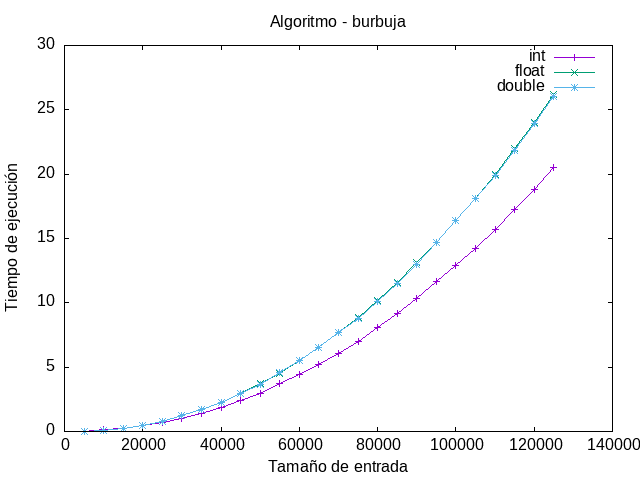
\includegraphics[width=\linewidth]{assets/Img/burbuja.png}
        \caption{Ejecución algoritmo burbuja}
        \label{fig:burbuja}
    \end{minipage}%
    \begin{minipage}{0.5\textwidth}
        \centering
        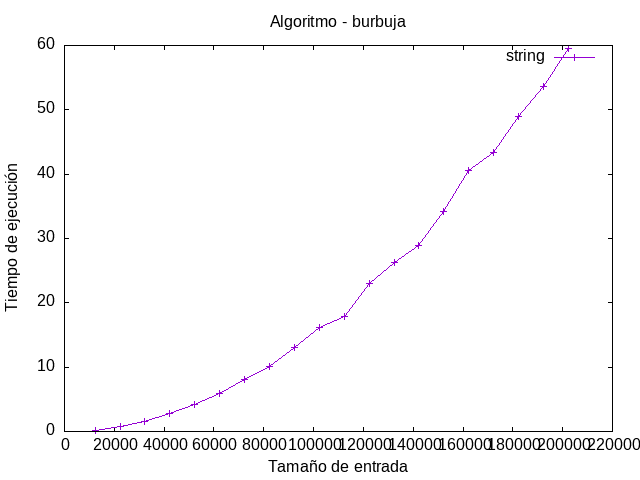
\includegraphics[width=\linewidth]{assets/Img/burbujastring.png}
        \caption{Ejecución algoritmo burbuja con string}
        \label{fig:burbujastring}
    \end{minipage}
\end{figure}
\subsection{Seleccion}
\begin{figure}[H]
    \begin{minipage}{0.5\textwidth}
        \centering
        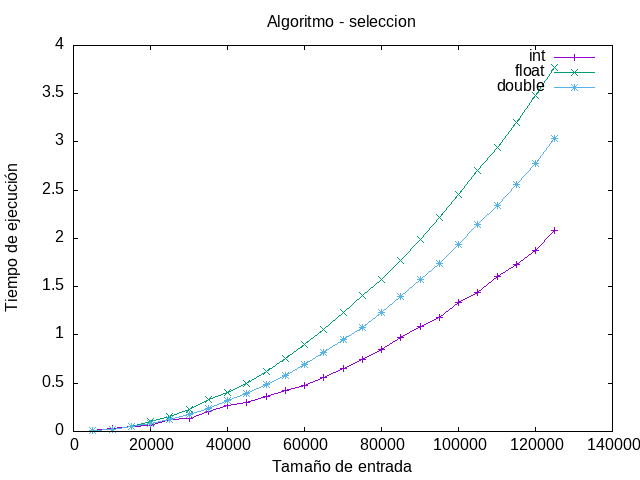
\includegraphics[width=\linewidth]{assets/Img/seleccion.png}
        \caption{Ejecución algoritmo seleccion}
        \label{fig:seleccion}
    \end{minipage}%
    \begin{minipage}{0.5\textwidth}
        \centering
        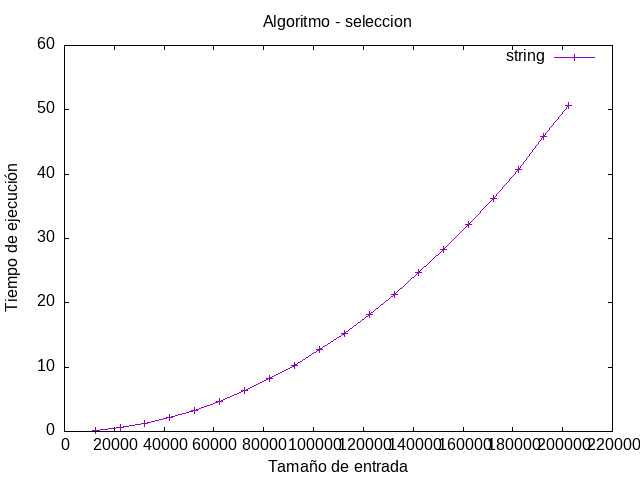
\includegraphics[width=\linewidth]{assets/Img/seleccionstring.png}
        \caption{Ejecución algoritmo seleccion con string}
        \label{fig:seleccionstring}
    \end{minipage}
\end{figure}

\subsection{Inserción}
\begin{figure}[H]
    \begin{minipage}{0.5\textwidth}
        \centering
        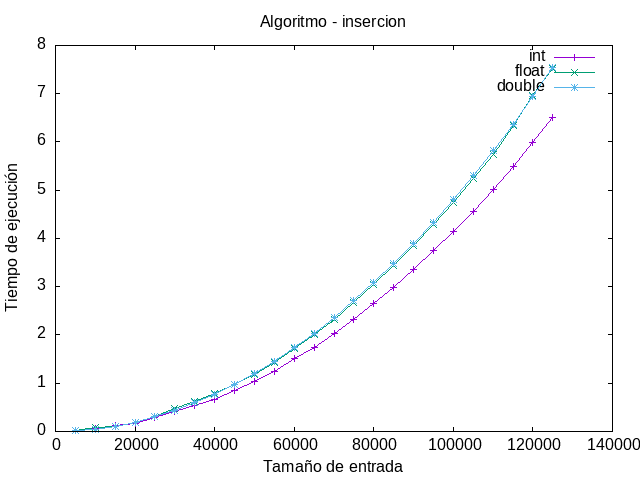
\includegraphics[width=\linewidth]{assets/Img/insercion.png}
        \caption{Ejecución algoritmo insercion}
        \label{fig:insercion}
    \end{minipage}%
    \begin{minipage}{0.5\textwidth}
        \centering
        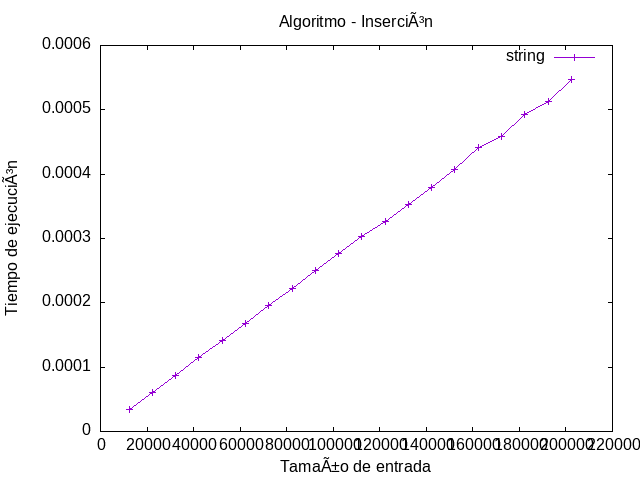
\includegraphics[width=\linewidth]{assets/Img/insercionstring.png}
        \caption{Ejecución algoritmo inserción con string}
        \label{fig:insercionstring}
    \end{minipage}
\end{figure}
\subsection{Hanoi}
\begin{figure}[H]
    \centering
        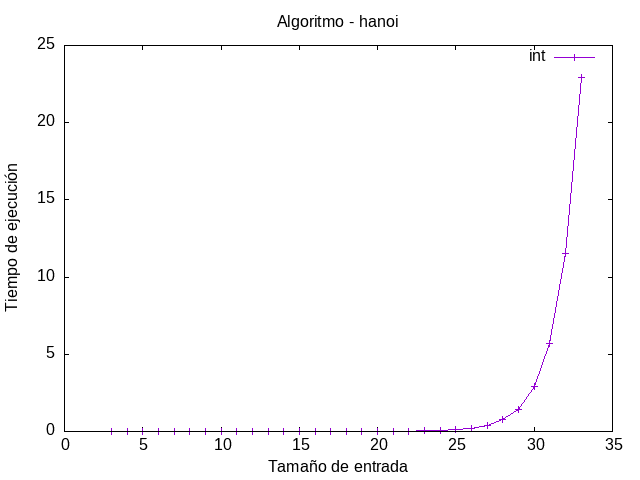
\includegraphics[width=0.5\linewidth]{assets/Img/hanoiint.png}
        \caption{Ejecución algoritmo Hanoi}
        \label{fig:hanoi}
\end{figure}
\subsection{Fibonacci}
\begin{figure}[H]
    \centering
        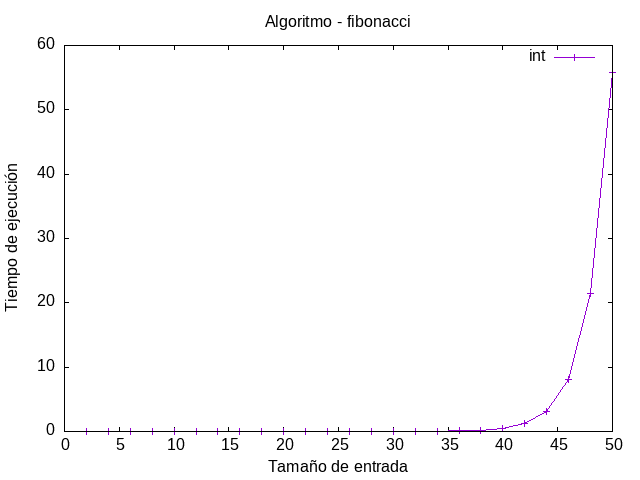
\includegraphics[width=0.5\linewidth]{assets/Img/fibonacciint.png}
        \caption{Ejecución algoritmo Fibonacci}
        \label{fig:fibonacci}
\end{figure}
\subsection{Floyd}
\begin{figure}[H]
    \centering
        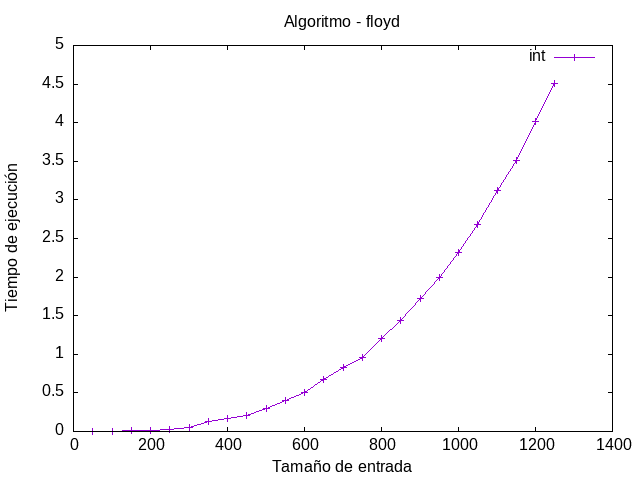
\includegraphics[width=0.5\linewidth]{assets/Img/floydint.png}
        \caption{Ejecución algoritmo Floyd}
        \label{fig:floyd}
\end{figure}
\section{Estudio de las gráficas}
    En esta sección se mostrarán las gráficas obtenidas en el estudio empírico de los algoritmos. 
    \subsection{Algoritmos  \(O(n^2)\)}
    Comenzaremos comparando las gráficas obtenidas para los algoritmos de ordenación con eficiencia \(O(n^2)\)
    \begin{figure}[H]
        \begin{minipage}{0.5\textwidth}
            \centering
            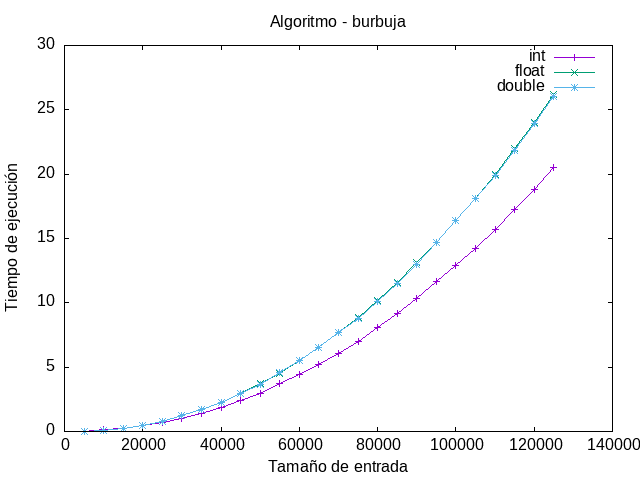
\includegraphics[width=\linewidth]{assets/Img/burbuja.png}
            \caption{Ejecución algoritmo burbuja}
            \label{fig:burbuja}
        \end{minipage}%
        \begin{minipage}{0.5\textwidth}
            \centering
            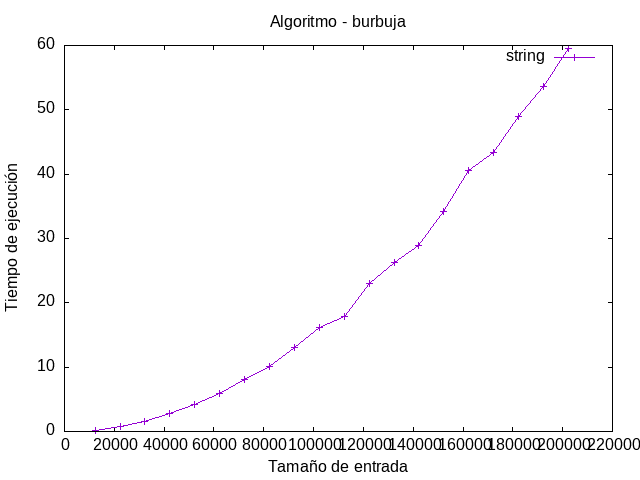
\includegraphics[width=\linewidth]{assets/Img/burbujastring.png}
            \caption{Ejecución algoritmo burbuja con string}
            \label{fig:burbujastring}
        \end{minipage}
    \end{figure}
    \begin{figure}[H]
        \begin{minipage}{0.5\textwidth}
            \centering
            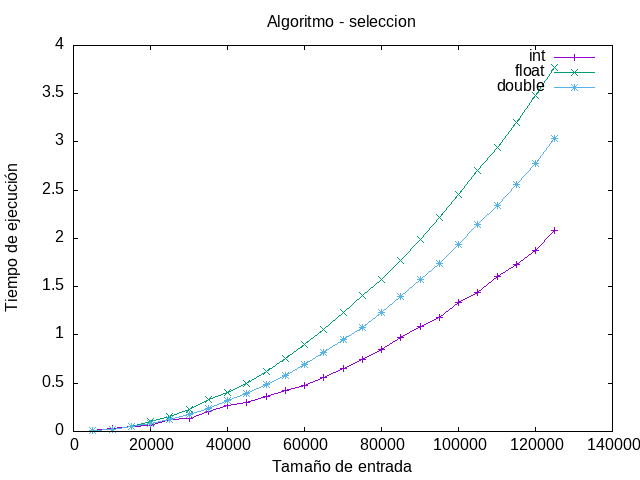
\includegraphics[width=\linewidth]{assets/Img/seleccion.png}
            \caption{Ejecución algoritmo seleccion}
            \label{fig:seleccion}
        \end{minipage}%
        \begin{minipage}{0.5\textwidth}
            \centering
            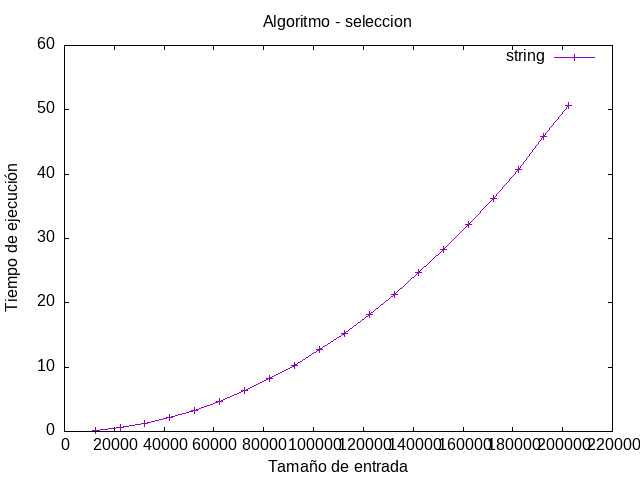
\includegraphics[width=\linewidth]{assets/Img/seleccionstring.png}
            \caption{Ejecución algoritmo seleccion con string}
            \label{fig:seleccionstring}
        \end{minipage}
    \end{figure}
    \begin{figure}[H]
        \begin{minipage}{0.5\textwidth}
            \centering
            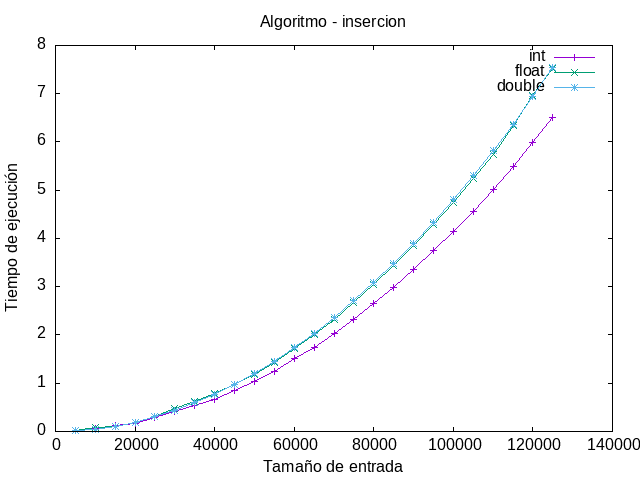
\includegraphics[width=\linewidth]{assets/Img/insercion.png}
            \caption{Ejecución algoritmo insercion}
            \label{fig:insercion}
        \end{minipage}%
        \begin{minipage}{0.5\textwidth}
            \centering
            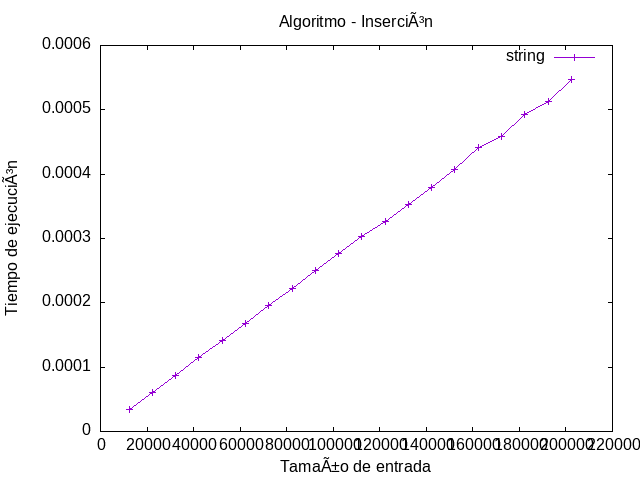
\includegraphics[width=\linewidth]{assets/Img/insercionstring.png}
            \caption{Ejecución algoritmo inserción con string}
            \label{fig:insercionstring}
        \end{minipage}
    \end{figure}
    Comenzaremos analizando primero los casos con tipos de datos int, float y double. Si nos fijamos en los tiempos de ejecución de cada algoritmo podemos ver que el algoritmo de burbuja es el que peor se comporta
    en todos los casos, seguido del algoritmo de Inserción y finalmente el algoritmo de selección. Dejando asi el algoritmo de burbuja como el peor de los tres y el de Inserción como el mejor.
    En el algoritmo de burbuja y de insercion se puede ver que el tiempo de ejecución es muy similar en todos los casos llegando a ser practicamente el mismo en los casos con datos double y float . 
    mientras que el algoritmo de seleccion si se ve mas afectado por el tipo de dato que se le pasa siendo los datos int los mas rápidos y los datos float los mas lentos.

    si nos fijamos en las graficas de los algoritmos con string podemos ver que los algoritmos de burbuja y seleccion son los que peor se comportan ya que se usa com entrada el libro del quijote en español lo 
    cual hace que haya muchas palabras repetidas y por tanto el algoritmo de burbuja y seleccion tengan que hacer mas comparaciones y por tanto mas tiempo de ejecución. En el caso del algoritmo de inserción
    vemos que esto le favorece y su tiempo de ejecución se reduce drasticamente en comparación con los datos int, float y double.
    \subsection{Algoritmos  \(O(n\log(n))\)}
    \begin{figure}[H]
        \begin{minipage}{0.5\textwidth}
            \centering
            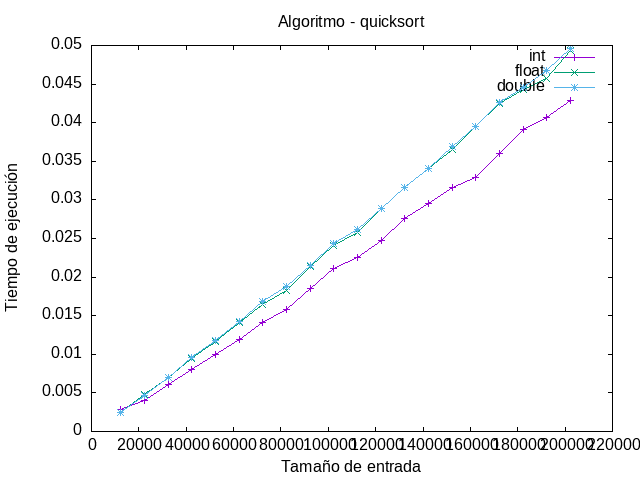
\includegraphics[width=\linewidth]{assets/Img/quicksort.png}
            \caption{Ejecución algoritmo insercion}
            \label{fig:quicksort}
        \end{minipage}%
        \begin{minipage}{0.5\textwidth}
            \centering
            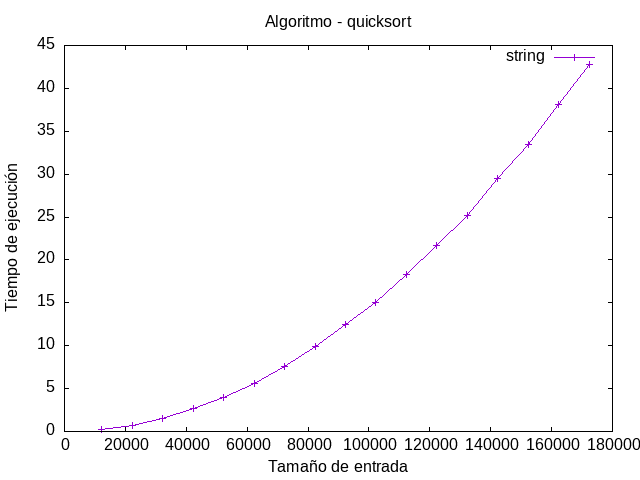
\includegraphics[width=\linewidth]{assets/Img/quicksortstring.png}
            \caption{Ejecución algoritmo inserción con string}
            \label{fig:quicksortstring}
        \end{minipage}
    \end{figure}
    \begin{figure}[H]
        \begin{minipage}{0.5\textwidth}
            \centering
            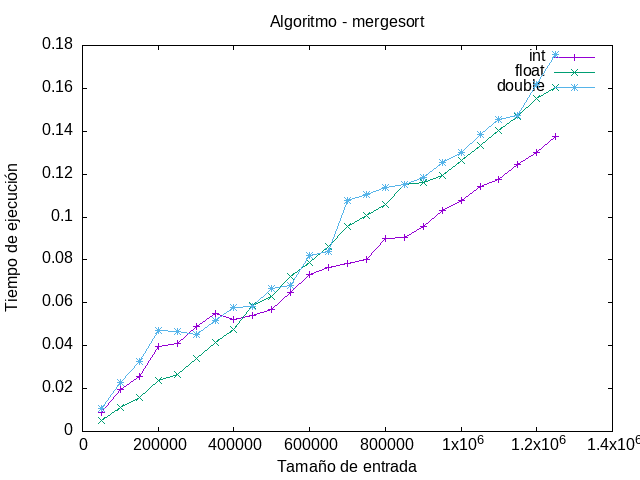
\includegraphics[width=\linewidth]{assets/Img/mergesort.png}
            \caption{Ejecución algoritmo mergesort}
            \label{fig:mergesort}
        \end{minipage}
    \end{figure}

    Pasamos ahora a estudiar los algoritmos con eficiencia \(O(n\log(n))\) los cuales veremos que son mas eficientes que los \(O(n^2)\)
    Si nos fijamos em la gráfica del quicksort veos que no hay casi diferencia entre los datos tipo float y double mientras que los datos tipo int son mas rapidos, 
    en el mergesort pasa justamente lo contrario , los tipos de datos double y float tardan menos en ser ordenados que los datos tipo int . 
    pero ambos son mas eficientes que los anteriormente vistos . 
    
    Si nos fijamos en las graficas de los algoritmos cuando los ejecutamos con datos de tipo string vemos que el mergesort gana en tiempo de ejecución al
    quicksort ya que en los casos donde hay datos repetidos el mergesort se comporta mejor que el quicksort debido a su implementacion.

    \subsection{Algoritmos Hanoi , Floyd y Fibbonaci}
    \begin{figure}[H]
        \begin{minipage}{0.5\textwidth}
            \centering
            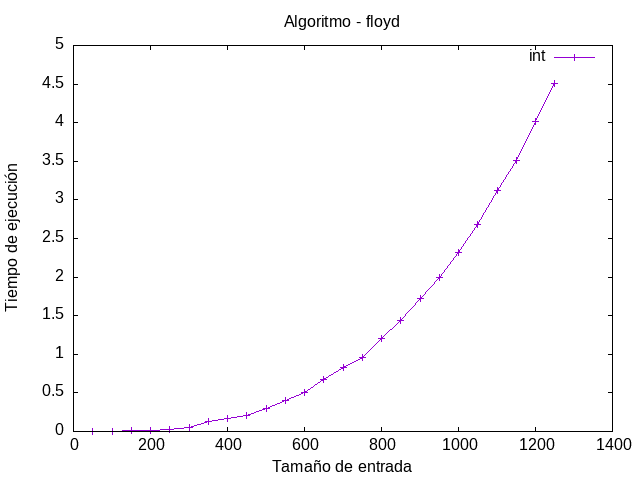
\includegraphics[width=\linewidth]{assets/Img/floydint.png}
            \caption{Ejecución algoritmo mergesort}
            \label{fig:mergesort}
        \end{minipage}
        \begin{minipage}{0.5\textwidth}
            \centering
            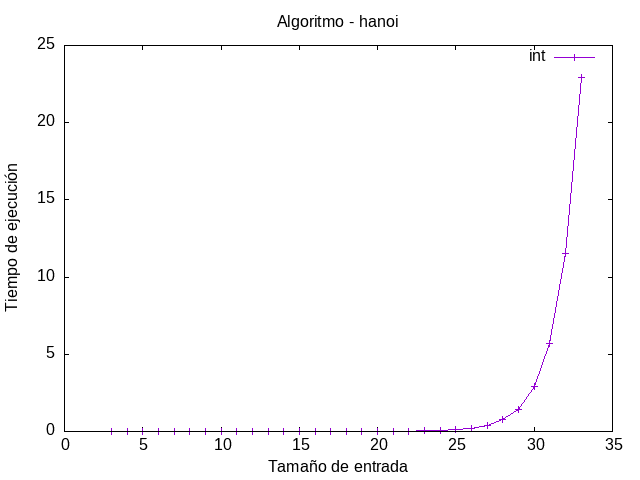
\includegraphics[width=\linewidth]{assets/Img/hanoiint.png}
            \caption{Ejecución algoritmo mergesort}
            \label{fig:mergesort}
        \end{minipage}
    \end{figure}
    \begin{figure}[H]
        \begin{minipage}{0.5\textwidth}
            \centering
            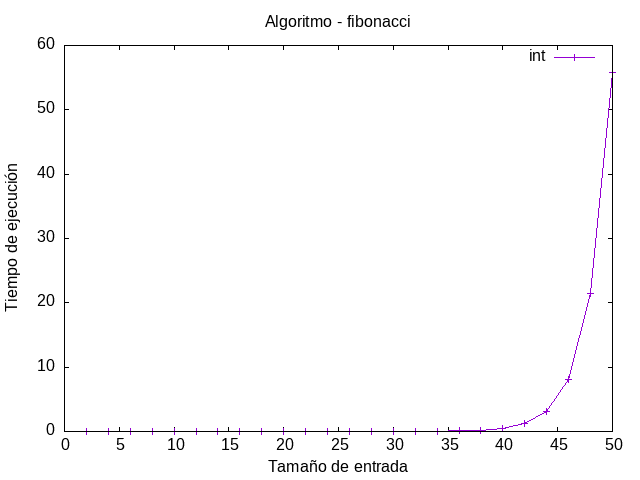
\includegraphics[width=\linewidth]{assets/Img/fibonacciint.png}
            \caption{Ejecución algoritmo mergesort}
            \label{fig:mergesort}
        \end{minipage}
    \end{figure}

    Por último pasamos a estudiar los algoritmos de Hanoi, Floyd y Fibonacci. Si nos fijamos en las gráficas de estos algoritmos vemos que el algoritmo de Floyd es el mas rapido ya que se trata de una algoritmo del orden \(O(n^3)\) por tanto 
    supera en velocidad a el algoritmo de Hanoi que es del orden \(O(2^n)\) y al algoritmo de Fibonacci que es del orden \(O((\frac{1+\sqrt{5}}{2})^n)\) siendo este ultimo el mas lento de todos.


    Como conclusion a este apartado hemos podido observar que los algoritmos de ordenación con eficiencia \(O(n^2)\) son mas lentos que los de eficiencia \(O(n\log(n))\) y que dependiendo del tipo de dato con el que se trabaje y de si hay datos repetidos o no habrá algoritmos a los que les afecte de manera 
    positiva como al mergesort o el de Inserción que pasa a ser practicamente logaritmico  y otros como el de burbuja o seleccion que se vean perjudicados por estos datos. 

\section{Conclusiones}

\end{document}